\documentclass{beamer}
\beamertemplatenavigationsymbolsempty
\usecolortheme{beaver}
\setbeamertemplate{blocks}[rounded=true, shadow=true]
\setbeamertemplate{footline}[page number]
%
\usepackage[utf8]{inputenc}
\usepackage[english]{babel}
\usepackage{amssymb,amsfonts,amsmath,mathtext}
\usepackage{subfig}
\usepackage[all]{xy} % xy package for diagrams
\usepackage{array}
\usepackage{multicol}% many columns in slide
\usepackage{hyperref}% urls
\usepackage{hhline}%tables
\usepackage{algorithmic}
\usepackage{algorithm}

\usepackage[backend=biber,style=authoryear]{biblatex}
\bibliography{../article/draft_lib} % assumes refs.bib includes the entry

% Your figures are here:
\graphicspath{ {fig/} {../figs/} }
\newcommand{\EE}{\mathbb{E}}
\newcommand{\R}{\mathbb{R}}
\newcommand{\eqdef}{\stackrel{\Delta}{=}}
\newcommand{\SG}{\mathrm{SG}}
\newcommand{\rd}[3]{\mathrm{D}_{#1}\infdivx*{#2}{#3}}
\newcommand{\rdalpha}[2]{\mathrm{D}_{\alpha}\infdivx*{#1}{#2}}
\newcommand{\renyi}{R\'enyi}
\newcommand{\erfc}{\mathrm{erfc}}
\newcommand{\eps}{\varepsilon}
\usepackage{mathtools}
\DeclarePairedDelimiterX{\infdivx}[2]{(}{)}{#1\;\delimsize\|\;#2}
%----------------------------------------------------------------------------------------------------------
\title[\hbox to 56mm{Feature generation}]{Differentially private modification of SignSGD}
\author[A.\,Yu.~Kravatskiy]{Alexey Kravatskiy}
\institute{Moscow Institute of Physics and Technology}
\date{\footnotesize
\par\smallskip\emph{Course:} My first scientific paper\par (Strijov's practice) \& Innovative Practicum /Group 205
\par\smallskip\emph{Expert:} A.\,N.~Beznosikov
\par\smallskip\emph{Consultant:} S.\,A.~Chezhegov
\par\bigskip\small 2025}

%----------------------------------------------------------------------------------------------------------
\begin{document}
%----------------------------------------------------------------------------------------------------------
\begin{frame}
\thispagestyle{empty}
\maketitle
\end{frame}
%-----------------------------------------------------------------------------------------------------
\begin{frame}{Distributed, Private, and Noise-resistant}
\begin{block}{Goal}
A communication-efficient and private algorithm for distributed optimization converging under heavy-tailed noise (noise with unbounded variance).
\end{block}
\begin{block}{Problem}
The only proposed private sign-based algorithm DP-SignSGD either is not private or does not converge.
\end{block}
\begin{block}{Solution}
A new privacy accountant for DP-SignSGD that affords lower noise to ensure privacy.
\end{block}
\end{frame}
%-----------------------------------------------------------------------------------------------------
\begin{frame}{Differential privacy of DP-SignSGD}

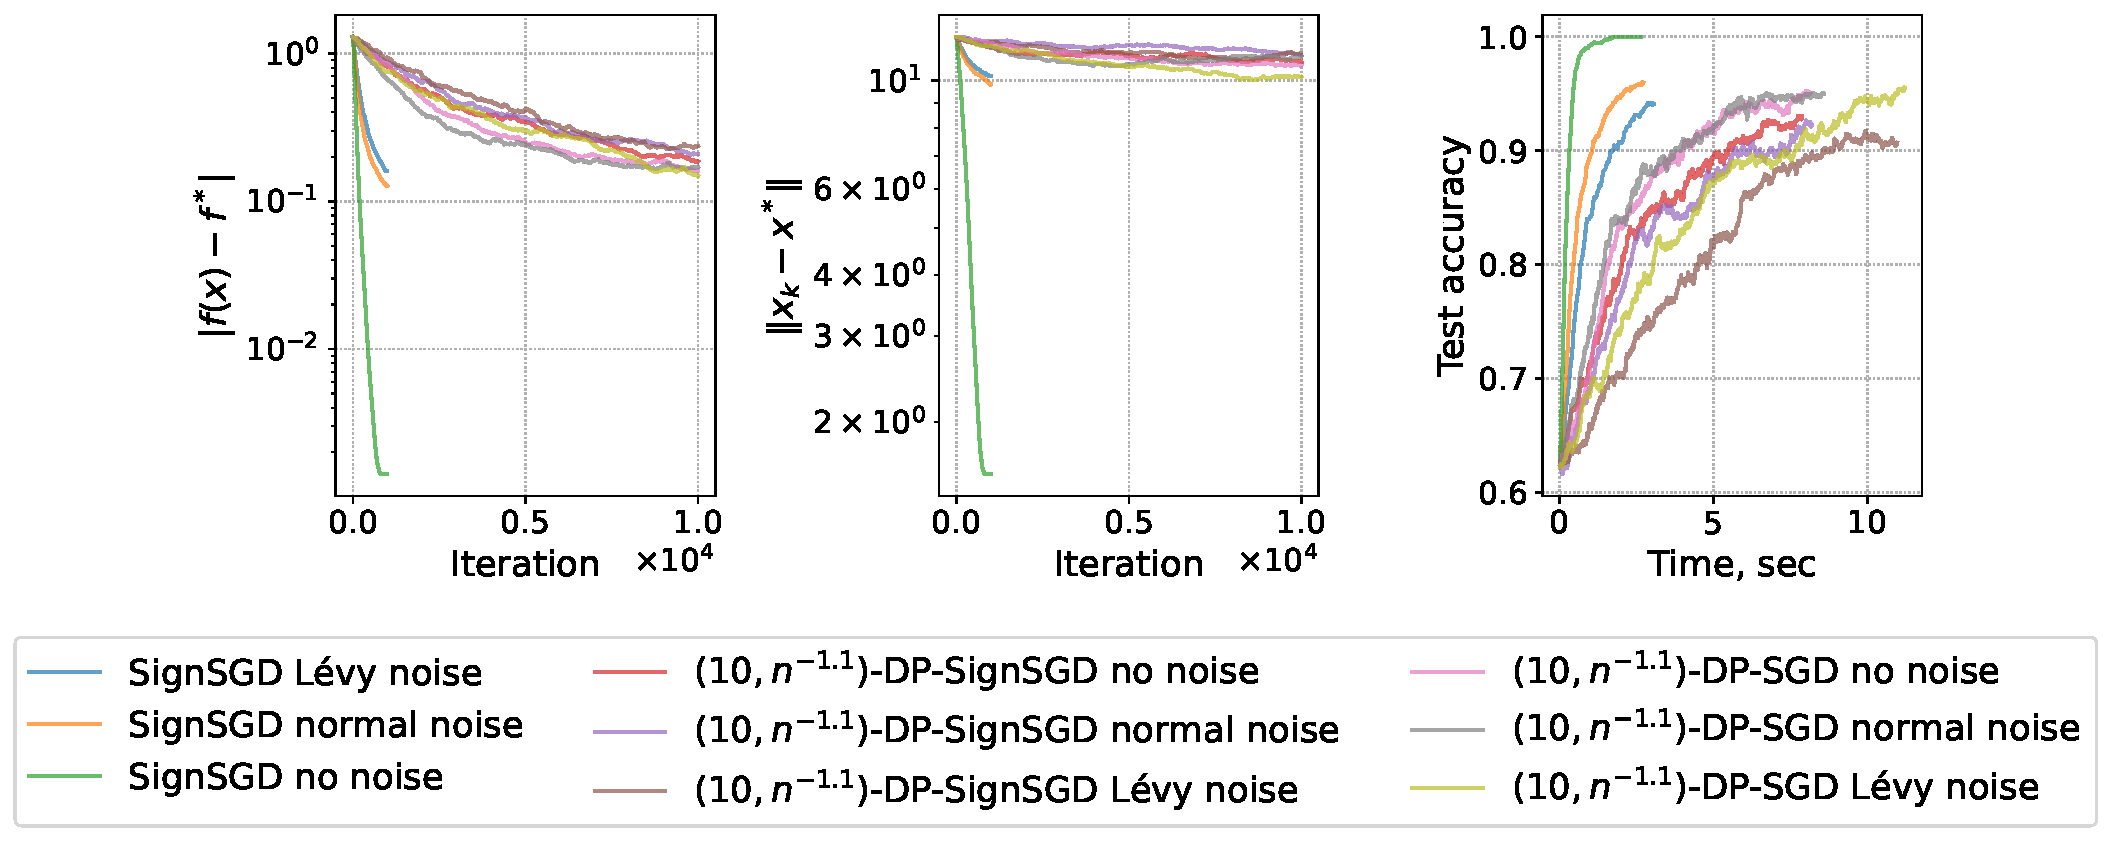
\includegraphics[width=1.0\textwidth]{v28_constant_step/short/v28_constant_step_short.pdf} 

\bigskip
DP-SignSGD with our DP-SIGN compressor is {\color{red} $(\eps, \delta)$-private and converges under heavy-tailed noise}. It behaves very much like DP-SGD with the same privacy mechanism.
\end{frame}

%-----------------------------------------------------------------------------------------------------
\begin{frame}{Literature}
\nocite{Jin2020}
\nocite{Mironov2017}
\nocite{mironov2019SGM}
\printbibliography
\end{frame}

%----------------------------------------------------------------------------------------------------------
\begin{frame}{Differential Privacy}
    \begin{definition}
        Given a set of local datasets $\mathcal{D}$ provided with a notion of neighboring local datasets $\mathcal{N}_{\mathcal{D}}\subset \mathcal{D}\times \mathcal{D}$ that differ in only one data point. For a query function $f: \mathcal{D}\rightarrow \mathcal{X}$, a mechanism $\mathcal{M}:\mathcal{X}\rightarrow \mathcal{O}$ to release the answer of the query is defined to be $(\epsilon,\delta)$-locally differentially private if for any measurable subset $\mathcal{S}\subseteq\mathcal{O}$ and two neighboring local datasets $(D_1,D_2)\in \mathcal{N}_{\mathcal{D}}$,
        $$
        P(\mathcal{M}(f(D_1))\in \mathcal{S}) \leq e^{\epsilon}P(\mathcal{M}(f(D_2))\in \mathcal{S}) + \delta.
        $$
    \end{definition}
        
        A key quantity in characterizing local differential privacy for many mechanisms is the sensitivity of the query $f$ in a given norm $l_{r}$, which is defined as
        $$
        \Delta_{r} = \max_{(D_1,D_2)\in\mathcal{N}_{\mathcal{D}}}||f(D_1)-f(D_2)||_r.
        $$
\end{frame}
%-----------------------------------------------------------------------------------------------------
\begin{frame}{Incorrect version of DP-SIGN (\cite{Jin2020})}
\begin{definition}
    For any given gradient $\boldsymbol{g}_{m}^{(t)}$, the compressor $\mathrm{dp\text{-}sign}$ outputs $\mathrm{dp\text{-}sign}(\boldsymbol{g}_{m}^{(t)},\epsilon,\delta)$. The $i$-th entry of $\mathrm{dp\text{-}sign}(\boldsymbol{g}_{m}^{(t)},\epsilon,\delta)$ is given by
    $$
    \mathrm{dp\text{-}sign}(\boldsymbol{g}_{m}^{(t)},\epsilon,\delta)_{i} =
    \begin{cases}
    1, & \text{with probability } \Phi\left(\dfrac{(\boldsymbol{g}_{m}^{(t)})_{i}}{\sigma}\right) \\[1.5ex]
    -1, & \text{with probability } 1-\Phi\left(\dfrac{(\boldsymbol{g}_{m}^{(t)})_{i}}{\sigma}\right)
    \end{cases}
    $$
    where $\Phi(\cdot)$ is the cumulative distribution function of the standard normal distribution; $\sigma = \dfrac{\Delta_{2}}{\epsilon}\sqrt{2\ln\left(\dfrac{1.25}{\delta}\right)}$, where $\epsilon$ and $\delta$ are the differential privacy parameters and $\Delta_2$ is the sensitivity measure.
\end{definition}
\end{frame}
%-----------------------------------------------------------------------------------------------------
\begin{frame}{Theorem 6 from (\cite{Jin2020})}
\begin{theorem}\label{dp-sign-probabilities}
    Let $u_{1},u_{2},\cdots,u_{M}$ be $M$ known and fixed real numbers. Further define random variables $\hat{u}_{i}=dp\text{-}sign(u_{i},\epsilon,\delta), \forall 1\leq i \leq M$. Then there always exist a constant $\sigma_{0}$ such that when $\sigma \geq \sigma_{0}$, $P(sign(\frac{1}{M}\sum_{m=1}^{M}\hat{u}_{i})\neq sign(\frac{1}{M}\sum_{m=1}^{M}u_{i})) <\big(1-x^2\big)^{\frac{M}{2}}$,
    where $x = \frac{|\sum_{m=1}^{M}u_{m}|}{2\sigma M}$.
\end{theorem}

\bigskip

\textcolor{red}{\textbf{Fault}} From the proof, it follows that the constant $\sigma_0$ depends on the values of $\{u_{i}\}$, which precludes from constructing DP-SIGN compressor.

\textcolor{red}{\textbf{Fault}} The authors have not guaranteed the overall $(\eps, \delta)$-privacy.

\textcolor{red}{\textbf{Fault}} The authors have not proved the convergence of their DP-SignSGD.


\end{frame}
%-----------------------------------------------------------------------------------------------------
\begin{frame}{Rényi divergence (\cite{Mironov2017})}
    \begin{definition}[\renyi\ divergence] Let $P$ and $Q$ be two distributions on $\mathcal{X}$ defined over the same probability space, and let $p$ and $q$ be their respective densities. The \renyi\ divergence of a finite order $\alpha\neq 1$ between $P$ and $Q$ is defined as
        \[
        \rdalpha{P}{Q}\eqdef \frac1{\alpha-1}\ln \int_{\mathcal{X}} q(x)\left(\frac{p(x)}{q(x)}\right)^{\alpha}\,\mathrm{d}x.
        \]
        \renyi\ divergence at orders $\alpha=1,\infty$ are defined by continuity.
        \end{definition}
    
\end{frame}
%-----------------------------------------------------------------------------------------------------
\begin{frame}{Rényi differential privacy (\cite{Mironov2017})}
    \begin{definition}[\renyi\ differential privacy (RDP)] We say that a randomized mechanism $\mathcal{M}\colon \mathcal{S}\to\mathcal{R}$ satisfies $(\alpha,\eps)$-\renyi\ differential privacy (RDP) if for any two \emph{adjacent} inputs $S,S'\in \mathcal{S}$ it holds that
        \[
        \rdalpha{\mathcal{M}(S)}{\mathcal{M}(S')}\leq \eps.
        \]
        \end{definition}
        
    
\end{frame}
%-----------------------------------------------------------------------------------------------------
\begin{frame}{Sample Gaussian Mechanism (\cite{mironov2019SGM})}
    \begin{definition}[Sampled Gaussian Mechanism (SGM)] Let $f$ be a function mapping subsets of $\mathcal{S}$ to $\mathbb{R}^d$. We define the Sampled Gaussian mechanism (SGM) parameterized with the sampling rate $0<q\leq 1$ and the noise $\sigma>0$ as
        \[
        \SG_{q,\sigma}(S)\eqdef f(\{x\colon x\in S \textrm{ is sampled with probability } q\})+\mathcal{N}(0,\sigma^2\mathbb{I}^d),
        \]
    where each element of $S$ is sampled independently at random with probability $q$ without replacement, and $\mathcal{N}(0,\sigma^2\mathbb{I}^d)$ is spherical $d$-dimensional Gaussian noise with per-coordinate variance $\sigma^2$.
    \end{definition}
    
    \end{frame}
%-----------------------------------------------------------------------------------------------------
\begin{frame}{Criterion of a private algorithm}
Following the procedure from \cite{mironov2019SGM}, we get:
$$\eps_R = \frac{1}{\alpha - 1} \log\left(\sum_{k=0}^{\alpha} {\alpha \choose k}  (1-q)^{\alpha-k}q^{k} \exp\left(\frac{k^2 - k}{2\sigma^2}\right)\right)$$

While according to the advanced composition theorem and conversion from \renyi\ privacy to $(\eps, \delta)$-privacy, $\eps_R$ must satisfy:
$$ \eps_R \leq \eps/T - \frac{\log 1/\delta}{T(\alpha - 1)}$$.
\end{frame}

%----------------------------------------------------------------------------------------------------------
\begin{frame}{Grid Search to find minimal $\sigma$}
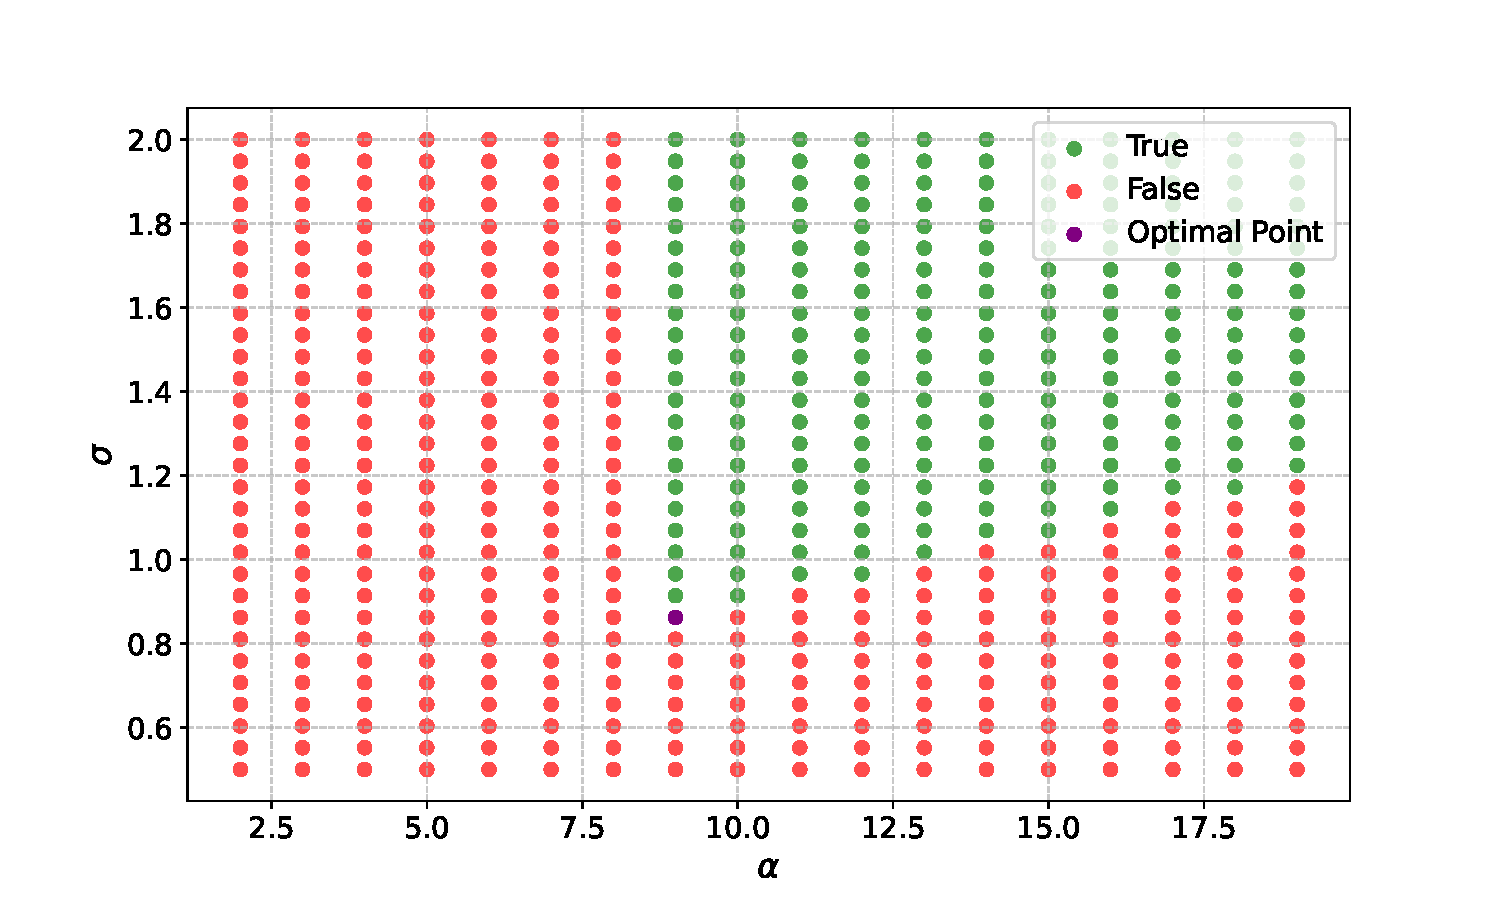
\includegraphics[width=1.0\textwidth]{grid_sigma_to_pres.pdf}
($\alpha$, $\sigma$) that guarantee ($\epsilon$, $\delta$)-dp of $T$ subsamplings for $\epsilon = 1$, $\delta = 1/n^{1.1}$, $T = 1000$, $q = 1/n$, where $n=649$ (10\% of the Mushroom dataset).

\end{frame}
%----------------------------------------------------------------------------------------------------------
\begin{frame}{Our version of DP-SIGN compressor}
\newcommand{\gradg}{\boldsymbol{g}}
    %\caption{DP-SIGN compressor}
    %\label{dp-sign-precise}
    \begin{algorithmic}
        \STATE \textbf{Input}: coordinate $w$, loss function $l$, user database $D$, $(\eps, \delta)$-privacy requirement, number of iterations $T$, sampling rate $q$, clipping level $C$.
        \STATE Prepare subsample $S$: add each element $(x, y) \in D$ with probability $q$.
        \STATE Compute the gradient $\gradg$ of the subsample: $\frac{1}{|S|}\sum_{(x,y)\in S}l(w;(x,y))$. If $S$ is empty, let $\gradg = 0$.
        \STATE If $||\gradg||_2 > C$: $\gradg = C\frac{\gradg}{||\gradg||_2}$.
        \STATE Grid search $\sigma(q, T, \eps, \delta)$ that satisfies 2 expressions for $\eps_R$ stated earlier.
        \STATE $\gradg_{priv}$ = $\gradg + \mathcal{N}(0,(C\sigma)^2\mathbb{I}^d)$
        \STATE \textbf{Output}: $sign(\gradg_{priv})$
    \end{algorithmic}
\end{frame}
%----------------------------------------------------------------------------------------------------------
\begin{frame}{UCI Mushroom Dataset}
There are 6,449 training samples equally distributed over 10 workers. Test consists of 1,625 samples. Each sample has $d = 112$ features. $q = 1/n$.

We solve the binary classification problem with $\lambda = 10^{-3}$ regularization.

\bigskip

Optimization problem:
$$\min_{x \in \mathbb{R}^n} \left( \frac{1}{m} \sum_{i=1}^m \ln(1 + \exp(-b_i \langle a_i, x \rangle)) + \frac{\lambda}{2} \|x\|^2 \right)
$$

Classification rule:
$b(a) := \text{sign}(\langle a, x \rangle)$

\bigskip

For each algorithm (SignSGD, DP-SGD, and DP-SignSGD), we set the learning rate $\eta=\frac{1}{\sqrt{100 d}}$. The goal is $(10, 1/n^{1.1})$ privacy.
\end{frame}
%-------------------------------------------------------------------------------------------------------
\begin{frame}{Heavy-tailed noise in gradient estimates}

    The unbiased estimate $\nabla f (x, \xi)$  has bounded $\kappa$-th moment $\kappa \in (1,2]$ for each coordinate, i.e., $\forall x \in \R^d$: 
    \begin{itemize}
        \item $\EE_\xi [\nabla f (x, \xi)] = \nabla f(x),$
        \item $\EE_\xi [|\nabla f (x, \xi)_i - \nabla f(x)_i|^\kappa] \leq \sigma_i^\kappa, i \in \overline{1,d},$
    \end{itemize}
    where $\Vec{\sigma} = [\sigma_1, \dots, \sigma_d]$ are non-negative constants.
    If $\kappa = 2$, then the noise is called a bounded variance. 

\end{frame}
%------------------------------------------------------------------------------------------------------
\begin{frame}{Synthetic heavy-tailed noise}
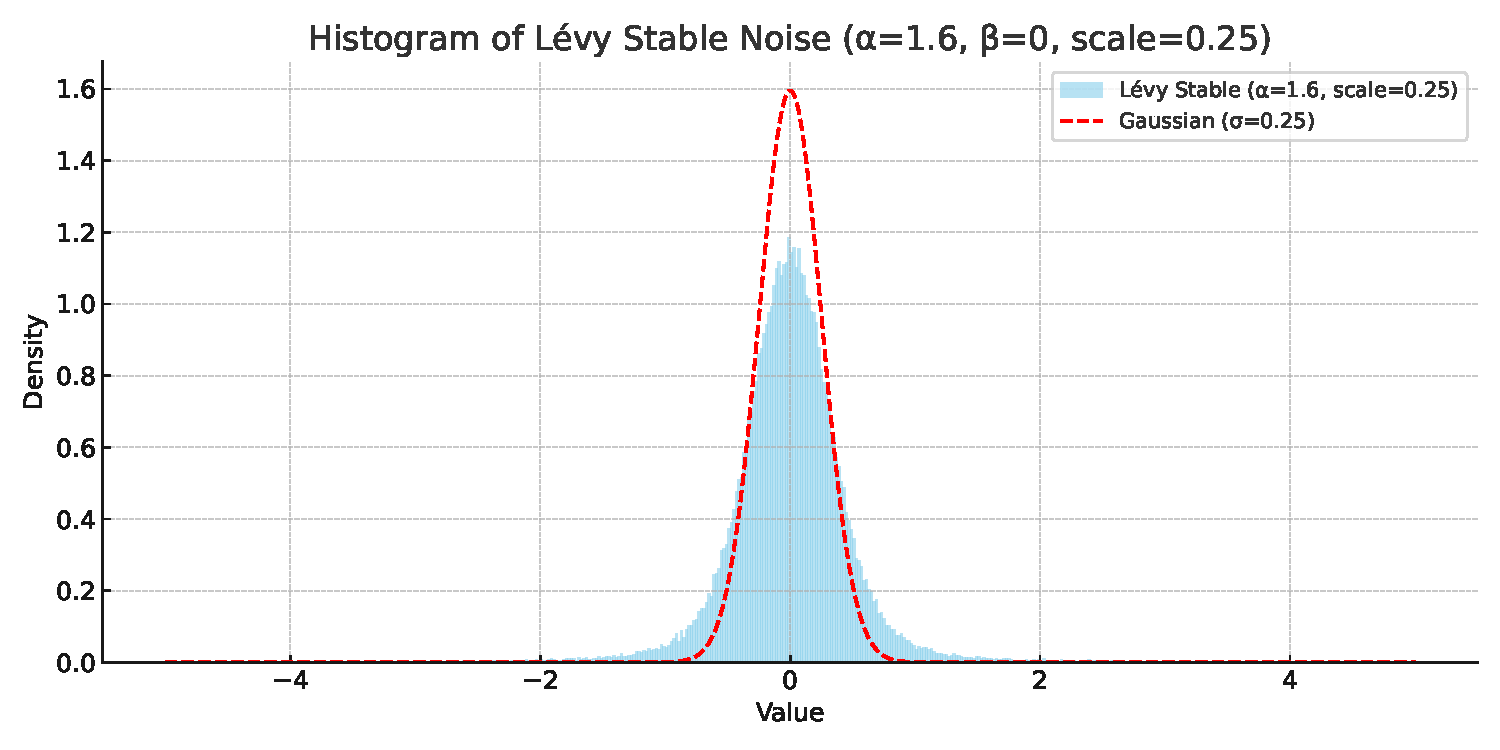
\includegraphics[width=1.0\textwidth]{levy_stable_histogram} 
We add to the gradients coordinatewise noise with Lévy stable distribution with $\sigma_l = 1/4$, $\alpha_l=1.6$, which corresponds to $\kappa=1.5$, and $\beta_l=0$ (this distribution is defined by its characteristic function $\varphi(t)=\exp\left(-0.25^{1.6}|t|^{1.6})\right)$.

We compare settings with no noise, $\mathcal{N}(0, 0.25^2\mathbb{I}^d)$ noise and this noise.
\end{frame}
%----------------------------------------------------------------------------------------------------------
\begin{frame}{Computational experiment}
    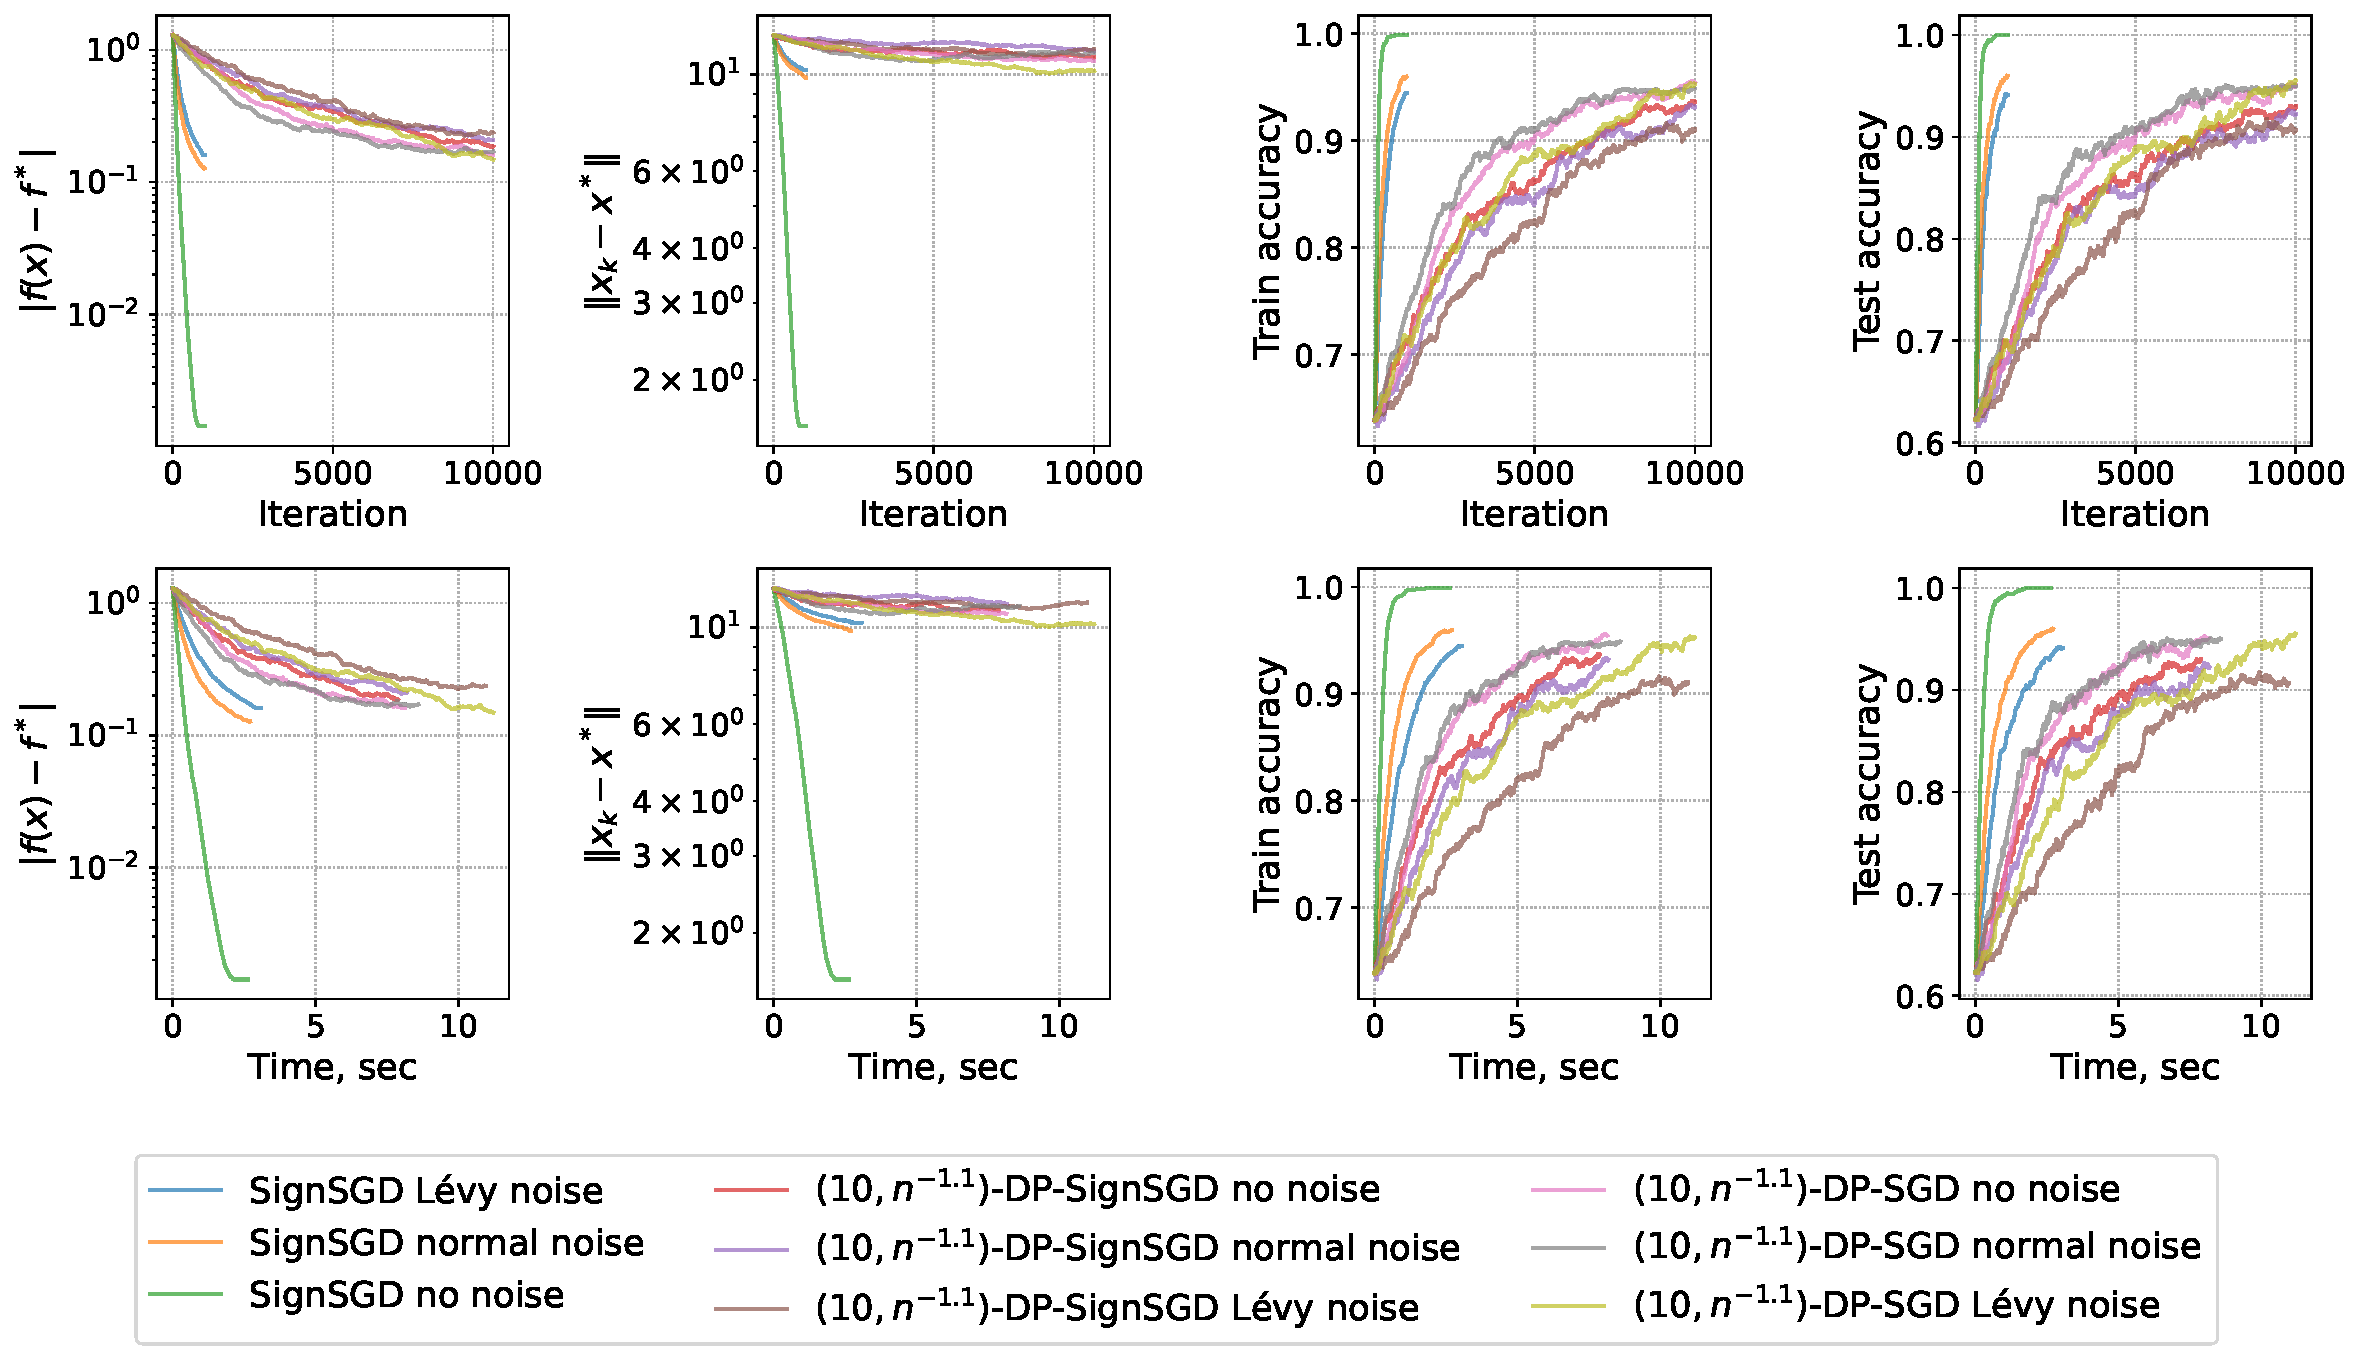
\includegraphics[width=1.0\textwidth]{v28_constant_step/long/v28_constant_step_long.pdf} 
DP-SignSGD converges very slowly, but it depends on a dataset. Lower $q$ leads to much lower $\sigma$ and better convergence.
\end{frame}
%----------------------------------------------------------------------------------------------------------
\begin{frame}{Constant vs Dynamic learning rate}
    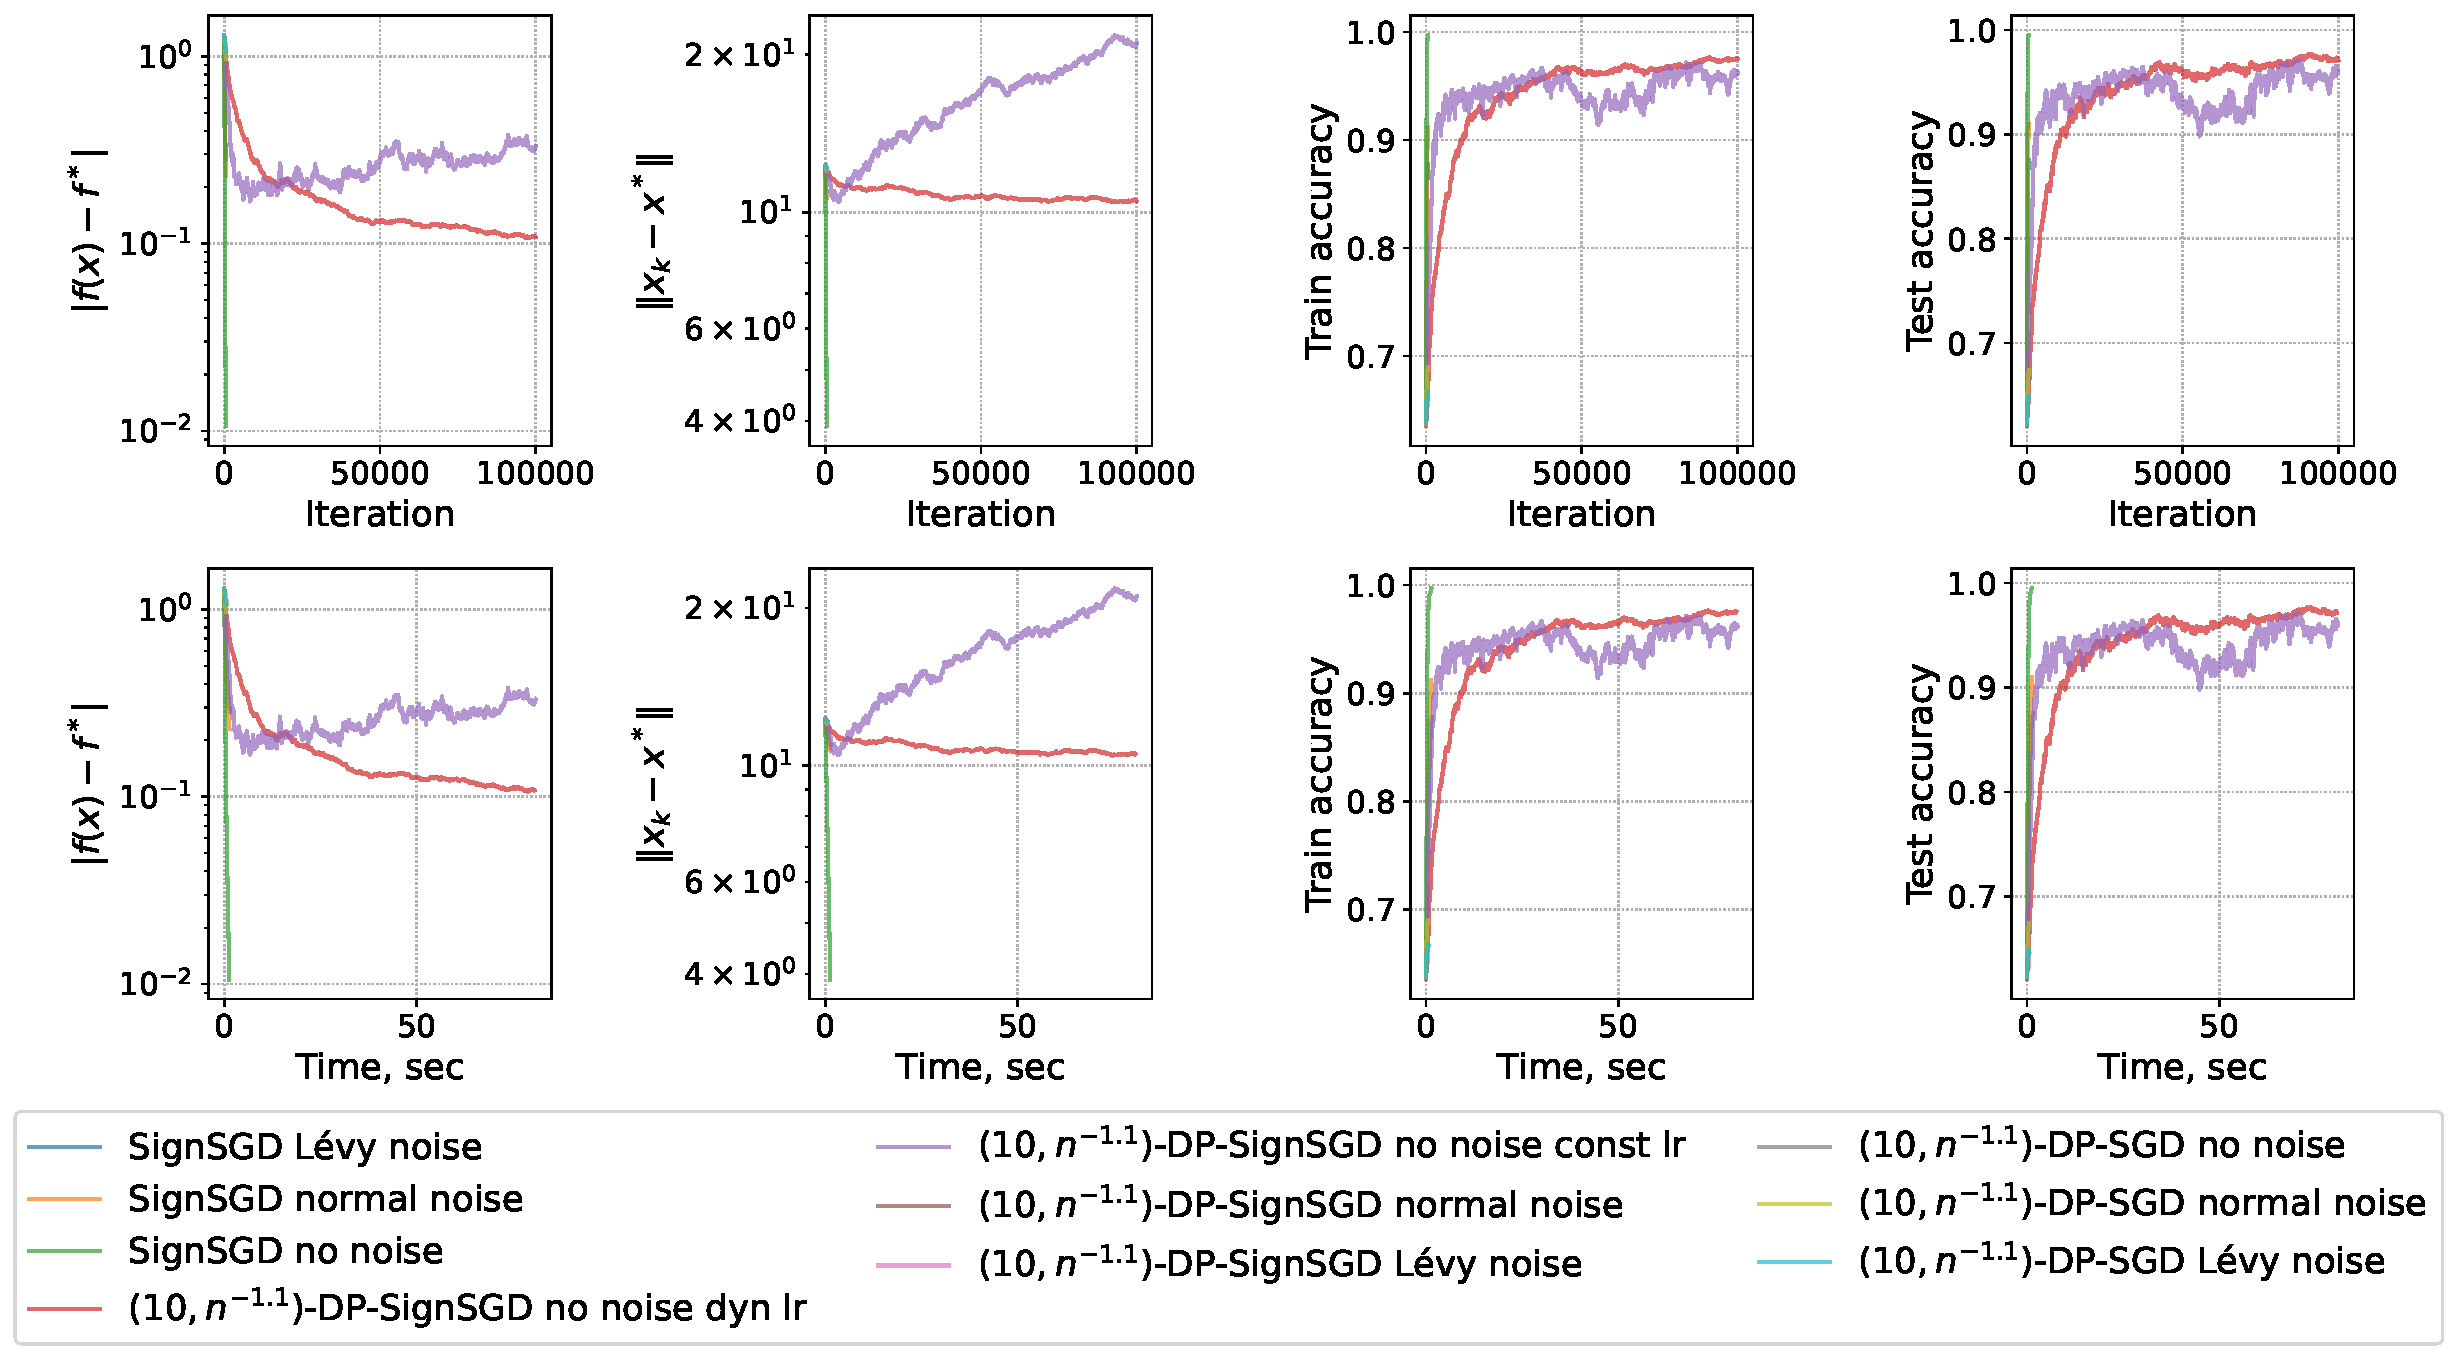
\includegraphics[width=1.0\textwidth]{v28_dynamic_step/long/v28_dynamic_step_long.pdf} 
DP-SignSGD converges better, when the learning rate is dynamic. $T^{-1/5}$ instead of $T^{-1/2}$ factor is required, because $\sigma$ depends on $T$.
\end{frame}
%----------------------------------------------------------------------------------------------------------
\begin{frame}{Our DP-SGD and DP-SignSGD are not feasible yet}
    \begin{figure}
        \centering
        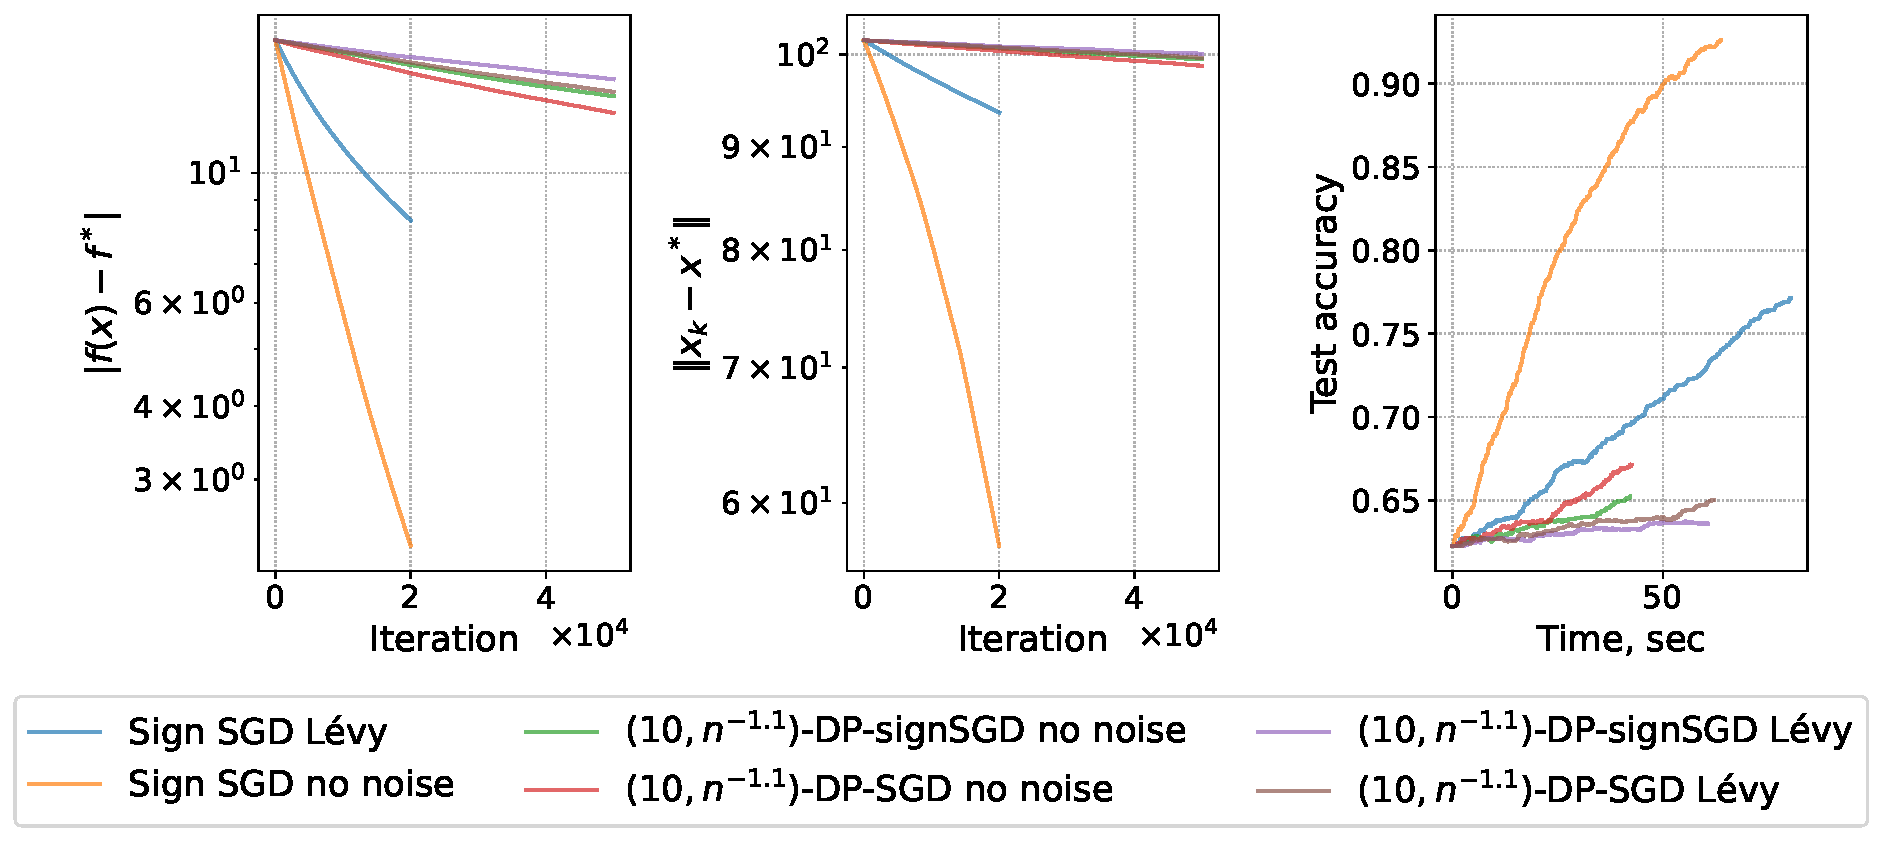
\includegraphics[width=1\textwidth]{v28_10eps_short.pdf}
    \end{figure}
    The current approach to construct DP-SGD might be not optimal: currently, our DP-SGD fails to converge on MLP problem.
\end{frame}
%----------------------------------------------------------------------------------------------------------
\begin{frame}{DP-SignSGD with Poisson sampling $q = 1/n$}
    \begin{itemize}
        \item $(10, 1/n^{1.1})$ differentially-private
        \item empirically converges on logistic regression problem even with heavy-tailed noise
        \item empirically converges with the same type of convergence like DP-SGD with Poisson subsampling
        \item benefits from slowly decreasing learning rate
    \end{itemize}
\end{frame}
%----------------------------------------------------------------------------------------------------------
\end{document} 